\chapter{Реализация и проверка приложения}

\section{Состав проекта и запуск}

Серверная часть содержит пять маршрутов HTTP и операции с SQLite. Настольный клиент выводит окно PySide6 и обрабатывает действия пользователя. Для установки библиотек предусмотрен файл зависимостей, для запуска на Windows используются командные файлы \path{START.bat}, \path{SERVER_ONLY.bat} и \path{CLIENT_OTHER_PC.bat}. Состав основных файлов приложения приведён в таблице \ref{tab:project-files}.

\begin{table}[H]
\caption{Основные файлы приложения}
\label{tab:project-files}
\small\centering\renewcommand{\arraystretch}{1.23}
\begin{tabularx}{\textwidth}{|L{53mm}|Y|}
\hline
Файл & Назначение \\
\hline
server.py & Сервер FastAPI и хранение задач в SQLite \\
\hline
client.py & Окно PySide6, список дел и обработка кнопок \\
\hline
requirements.txt & Библиотеки для установки на двух компьютерах \\
\hline
START.bat & Запуск сервера и двух клиентов на одном ПК \\
\hline
SERVER\_ONLY.bat & Запуск сервера на первом ПК \\
\hline
CLIENT\_OTHER\_PC.bat & Запуск клиента на втором ПК \\
\hline
README.txt & Инструкция по запуску \\
\hline
tasks.db & Файл SQLite с общим списком задач; создаётся при первом запуске \\
\hline
\end{tabularx}
\end{table}

На обоих компьютерах устанавливается Python и библиотеки из файла \path{requirements.txt}. На первом ПК командой \path{START.bat} запускаются сервер и два клиента для локальной проверки. Для работы в сети на первом ПК открывают \path{SERVER_ONLY.bat}, а на втором \path{CLIENT_OTHER_PC.bat} и вводят IP-адрес первого компьютера. Сам сервер использует порт 8000. Клиент первого ПК может обращаться к адресу \texttt{127.0.0.1}; второму нужен реальный локальный IPv4-адрес первого ПК.

Чтобы узнать адрес, на первом компьютере достаточно выполнить команду \texttt{ipconfig}. Во время работы оба компьютера должны находиться в одной локальной сети. Если сервер не открывается со второго ПК, нужно проверить адрес и правила брандмауэра Windows. Важно не запускать отдельный сервер на каждом компьютере: иначе программы окажутся подключены к разным базам, и синхронизации не будет.

После запуска сервера рядом с \texttt{server.py} создаётся файл \texttt{tasks.db}, если его ещё нет. В нём сохраняются названия задач и отметки их выполнения. После остановки сервера файл остаётся на диске. Когда сервер запускается снова, он открывает ту же базу. SQLite работает с файлом базы непосредственно, без отдельного сервера СУБД.

\section{Сервер и операции с данными}

Сервер FastAPI обрабатывает пять маршрутов. При чтении он выбирает записи из таблицы \texttt{tasks}; при добавлении вставляет строку; отдельный PATCH-запрос исправляет название, другой PATCH меняет отметку выполнения; DELETE удаляет запись. Перечень операций представлен в таблице \ref{tab:api}.

\begin{table}[H]
\caption{HTTP-операции сервера}
\label{tab:api}
\small\centering\renewcommand{\arraystretch}{1.22}
\begin{tabularx}{\textwidth}{|L{19mm}|L{40mm}|Y|}
\hline
Метод & Адрес & Назначение \\
\hline
GET & /tasks & Получить общий список задач \\
\hline
POST & /tasks & Добавить задачу \\
\hline
PATCH & /tasks/\{id\} & Поменять отметку выполнения \\
\hline
PATCH & /tasks/\{id\}/title & Исправить название задачи \\
\hline
DELETE & /tasks/\{id\} & Удалить выбранную задачу \\
\hline
\end{tabularx}
\end{table}

Для новой задачи клиент передаёт JSON-объект с полем \texttt{title}. FastAPI преобразует данные к модели \texttt{Task}, после чего запускается обработчик добавления \cite{fastapibody}. Он удаляет пробелы по краям и проверяет длину названия. Строка из одних пробелов и название длиннее 120 символов не записываются. Если ввод неверен, сервер возвращает HTTP 400 и сообщение об ошибке. Такая проверка нужна не только графическому окну: запрос может быть отправлен напрямую через страницу \texttt{/docs}.

Данные размещаются в одной таблице SQLite с полями \texttt{id}, \texttt{title}, \texttt{done}. Первичный ключ \texttt{id} генерируется автоматически. При добавлении выполняется SQL INSERT с параметром вместо подстановки пользовательского текста в запрос. Это позволяет хранить строки, содержащие кавычки и другие символы, без ручного формирования SQL-выражения \cite{pythonsqlite}. После сохранения сервер возвращает ответ, а клиент запрашивает обновлённый перечень.

Чтобы исправить название, клиент открывает диалог ввода и отправляет PATCH-запрос на адрес \texttt{/tasks/\{id\}/title}. На сервере применяется та же проверка текста, что при создании задачи. Меняется только поле \texttt{title}; первичный ключ и состояние остаются прежними. Когда пользователь выбирает задачу и нажимает кнопку изменения состояния, приложение отправляет другой PATCH-запрос с идентификатором. Сервер выполняет SQL UPDATE, переключающий число в поле \texttt{done} между 0 и 1. Чтобы изменить именно выбранную запись, используется условие \texttt{WHERE id = ?} \cite{pythonsqlite}. При удалении аналогичным образом выполняется SQL DELETE \cite{pythonsqlite}. Если идентификатор отсутствует, сервер возвращает ошибку HTTP 404.

При чтении списка выполняется запрос SELECT с сортировкой по идентификатору: новые задачи располагаются первыми. В ответе каждая запись содержит целочисленный идентификатор, название и логическую отметку выполнения. Клиент использует эти значения при построении списка. Ему не требуется знать расположение файла базы данных или выполнять SQL-запросы самостоятельно.

Блок \texttt{with sqlite3.connect} автоматически завершает транзакцию: сохраняет изменения при успешной операции и откатывает их при ошибке.

\section{Алгоритмы работы программы}

Алгоритм добавления задачи начинается с пользовательского ввода. После нажатия кнопки выполняется проверка названия. Пустую строку нельзя передать серверу как корректную задачу. Для остальных строк отправляется HTTP-запрос. Если соединение недоступно или сервер отвечает ошибкой, интерфейс сообщает об этом пользователю, не очищая введённый текст. При успешном ответе поле ввода очищается, затем выполняется чтение актуального списка. Последовательность приведена на рисунке \ref{fig:addtask}.

\begin{center}
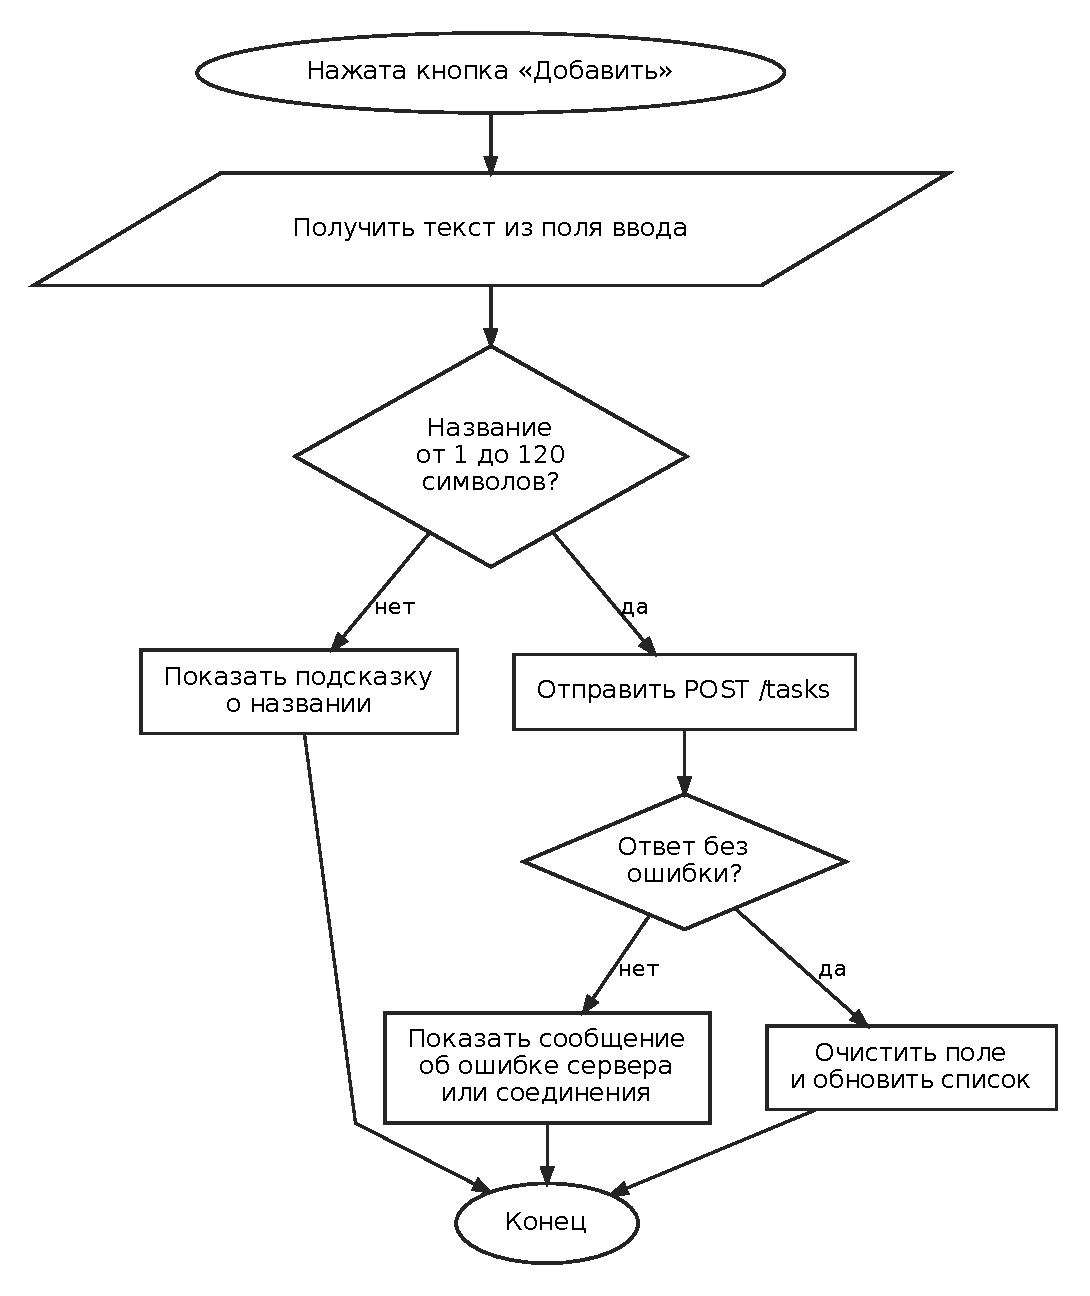
\includegraphics[width=.88\textwidth,height=.58\textheight,keepaspectratio]{figures/add.pdf}
\captionof{figure}{Последовательность добавления задачи и обработки ошибки}
\label{fig:addtask}
\end{center}

На блок-схемах эллипс обозначает начало и конец алгоритма, прямоугольник обозначает действие, а ромб обозначает проверку условия \cite{gostflow}. Ветви ошибки заканчиваются сообщением пользователю без добавления записи.

Редактирование названия показано на рисунке \ref{fig:edit}. Если задача не выбрана, пользователь получает подсказку. Нажатие «Отмена» закрывает диалог без изменений. Название проверяется перед отправкой PATCH-запроса; после успешного ответа клиент получает обновлённый список.

\begin{center}
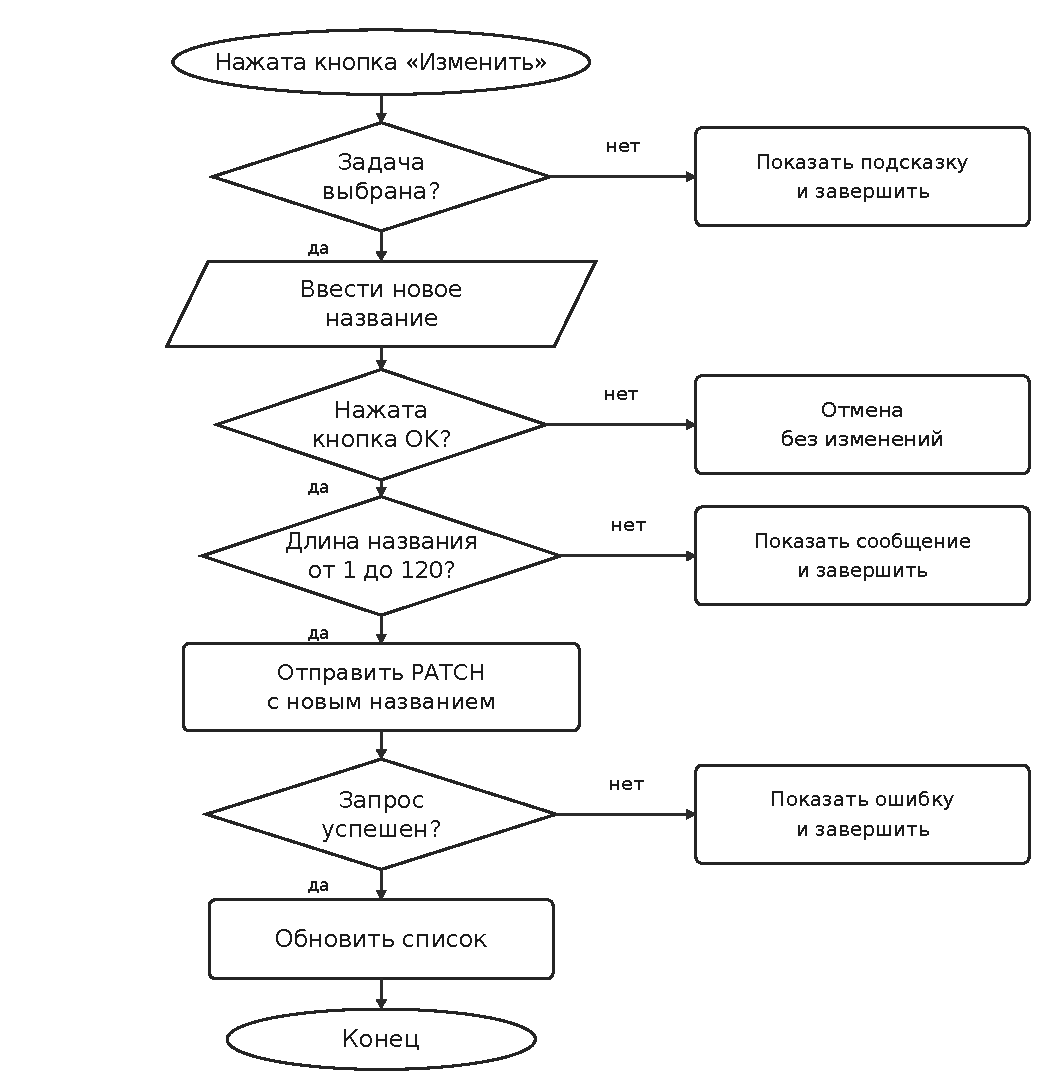
\includegraphics[width=.96\textwidth,height=.65\textheight,keepaspectratio]{figures/edit.pdf}
\captionof{figure}{Алгоритм изменения названия задачи}
\label{fig:edit}
\end{center}

Работа таймера показана на рисунке \ref{fig:sync}. Раз в две секунды клиент запрашивает список. Если данные изменились, он обновляет перечень и показатели статистики; иначе оставляет экран без изменений. Если чтение не удалось из-за отсутствия соединения, нижняя строка сообщает о потере связи. Ранее полученные записи остаются видимыми. При следующем срабатывании таймера запрос повторяется.

\begin{center}
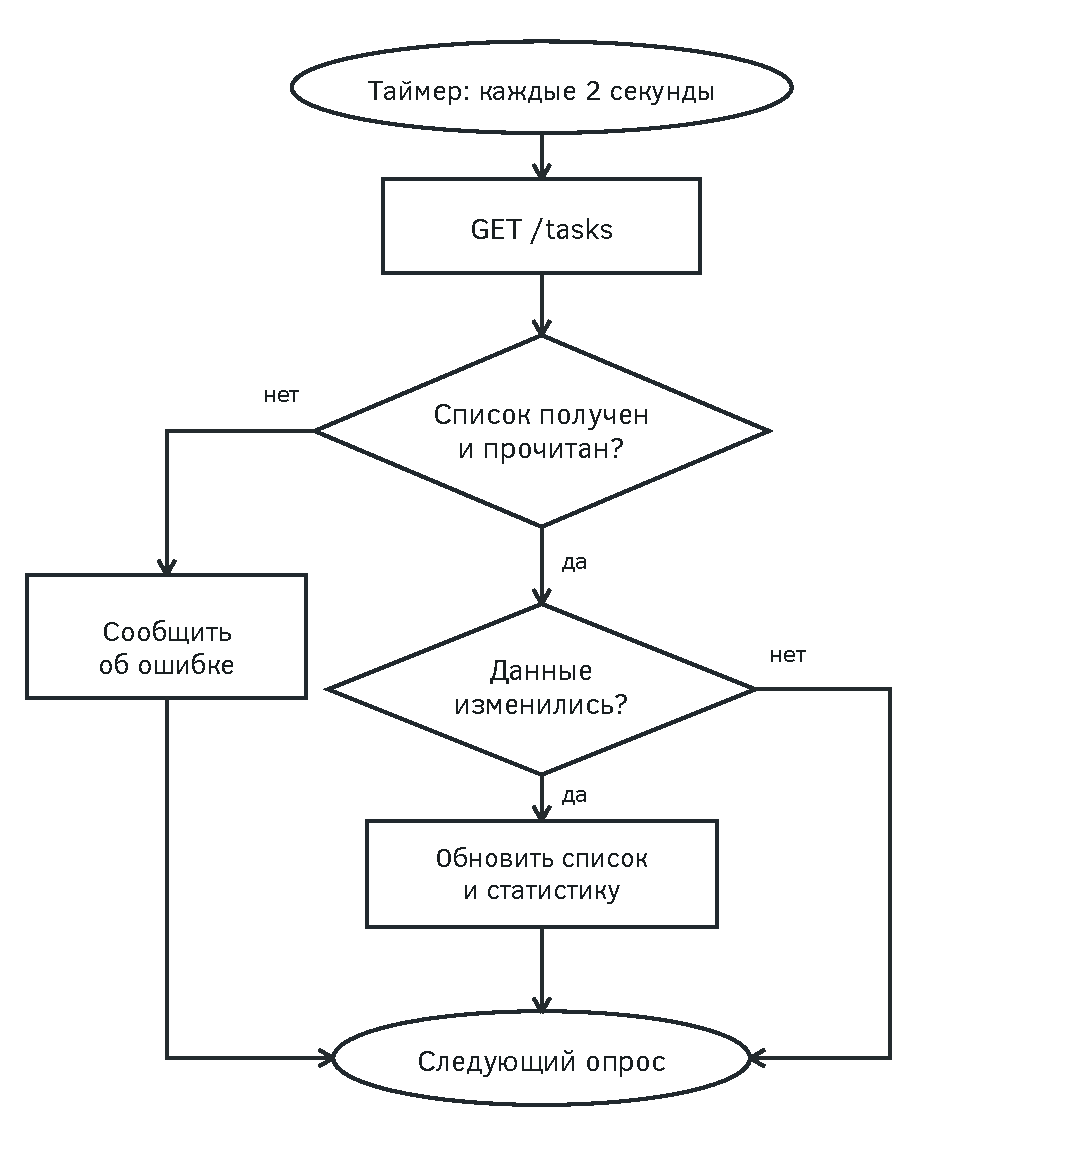
\includegraphics[width=.88\textwidth,height=.58\textheight,keepaspectratio]{figures/sync.pdf}
\captionof{figure}{Алгоритм периодического обновления списка задач}
\label{fig:sync}
\end{center}

Выбранная схема не требует отдельного канала уведомлений от сервера. Оба клиента сами обращаются за актуальными данными. У такого способа есть ограничение: фактическое появление изменения зависит от момента следующего опроса. Если задача была создана непосредственно после очередного запроса второго клиента, он увидит её только при следующем обращении. Таймер настроен на две секунды. Производительность и оптимальная частота запросов отдельно не измерялись.

При запуске окно отправляет запрос списка. При недоступном сервере появляется сообщение «Нет связи с сервером». При первом запуске экран остаётся пустым, а после временного отключения виден ранее полученный список. Если сервер вернул неверный JSON, окно также показывает сообщение об отсутствии связи. Очередной успешный запрос заменяет прежние данные.

Навигация между тремя страницами не затрагивает базу данных. Вкладки «Задачи», «Статистика» и «О программе» выбирают соответствующий экран. Для этого используется QTabWidget, который показывает нужную страницу в том же окне \cite{qttabs}. Состояние соединения и таймер принадлежат главному окну, поэтому переход на информационную страницу не останавливает периодическое обновление. При возвращении пользователь видит последнее полученное состояние задач.

Обработка кнопок строится на сигнале нажатия. Qt связывает действия пользователя с вызываемыми методами; для приложения на Python это обычные функции объекта окна. В отличие от самостоятельного цикла опроса клавиатуры, библиотека управляет событиями и вызывает нужный обработчик при нажатии. Обработка сигналов и событий относится к стандартной модели Qt \cite{prokhorenok,qtdocs}.

Алгоритм удаления проверяет выбранную строку прежде, чем отправить запрос. Идентификатор хранится внутри элемента списка как отдельные данные. Такое решение защищает от неоднозначности: два пункта могут иметь одинаковые названия, но разные идентификаторы. Операция выполняется именно над выбранной записью. Текст названия не используется для удаления, поэтому повторяющиеся формулировки задач не приводят к случайному изменению нескольких строк.

\section{Пользовательский интерфейс}

Главное окно содержит три вкладки: «Задачи», «Статистика» и «О программе». На вкладке «Задачи» расположены поле для названия, кнопка добавления, поиск, фильтр и список записей. Выбранную задачу можно переименовать, отметить выполненной, вернуть в работу или удалить. Кнопка «Сохранить TXT» записывает весь список в текстовый файл. На рисунке \ref{fig:taskwindow} показано главное окно программы в Windows.

\begin{figure}[htbp]
\centering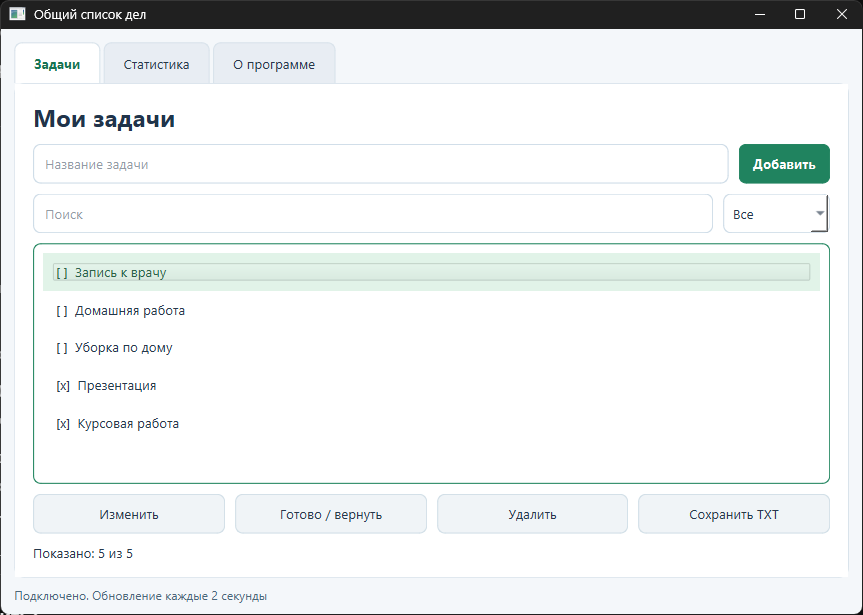
\includegraphics[width=.92\textwidth,height=.39\textheight,keepaspectratio]{figures/screenshots/tasks.png}
\caption{Окно приложения со списком задач}
\label{fig:taskwindow}
\end{figure}

Для поиска достаточно ввести часть названия. Фильтр «Все», «В работе» или «Выполнено» ограничивает видимые записи, но не изменяет данные на сервере. Перед названием показано [x] для выполненной задачи и [ ] для невыполненной. На снимке показаны пять задач, две из них отмечены выполненными. Среди записей есть «Запись к врачу», «Домашняя работа» и «Уборка по дому».

Редактирование выполняется через стандартный диалог ввода текста QInputDialog. Он открывается после выбора строки и нажатия кнопки «Изменить». На рисунке \ref{fig:editwindow} показано изменение названия первой задачи на «Запись к врачу в 19:00».

\begin{figure}[htbp]
\centering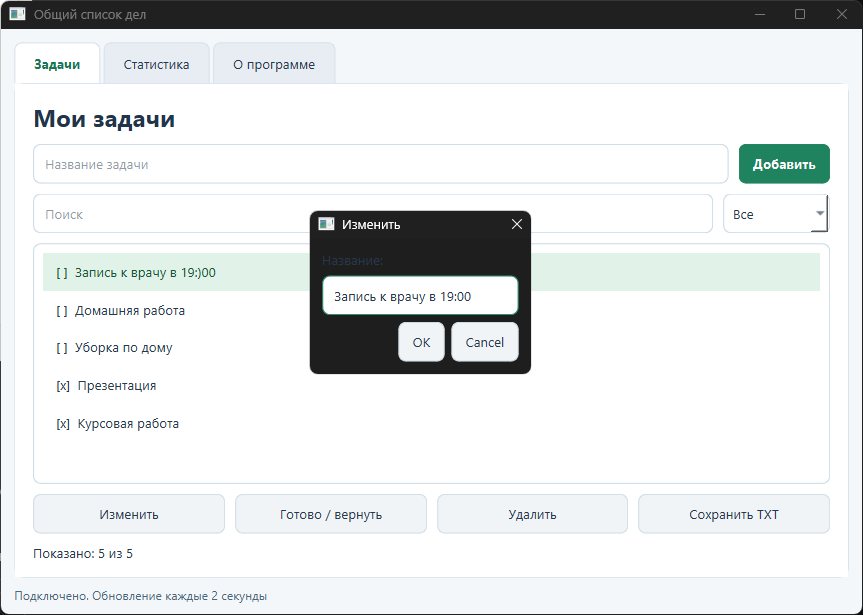
\includegraphics[width=.87\textwidth,height=.37\textheight,keepaspectratio]{figures/screenshots/edit.png}
\caption{Диалог изменения названия выбранной задачи}
\label{fig:editwindow}
\end{figure}

При пустом названии окно показывает подсказку. После подтверждения редактирования клиент отправляет запрос на сервер и перечитывает список. Если задача не выбрана, изменение не выполняется. Удаление также требует выбора записи и подтверждения действия.

На вкладке «Статистика» отображаются три числа: количество всех задач, задач в работе и выполненных. Шкала показывает долю выполненных. Значения рассчитываются из полученного списка; отдельного запроса к серверу для статистики нет. На рисунке \ref{fig:statswindow} показаны три блока статистики и шкала прогресса. В списке пять задач: три в работе и две выполнены, доля выполнения составляет 40\%.

\begin{figure}[htbp]
\centering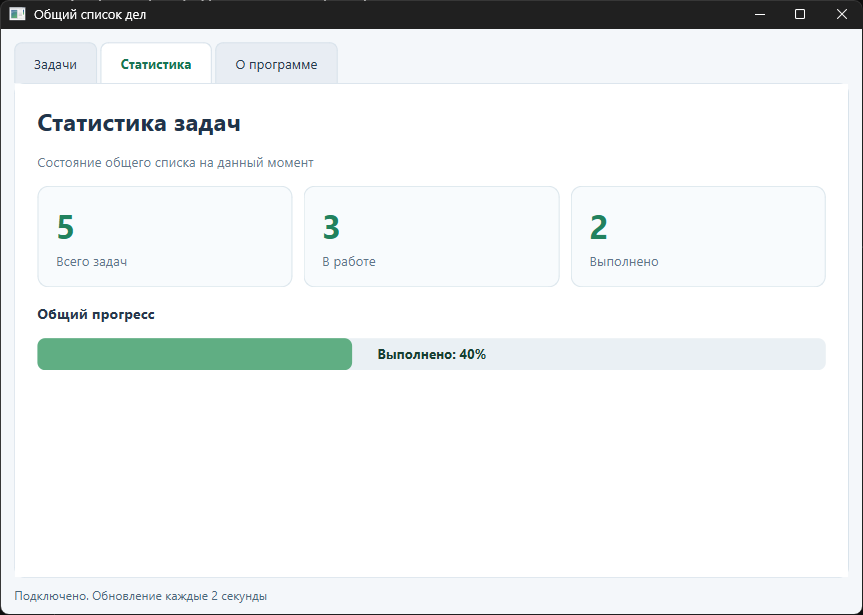
\includegraphics[width=.90\textwidth,height=.37\textheight,keepaspectratio]{figures/screenshots/stats.png}
\caption{Вкладка «Статистика» в работающем приложении}
\label{fig:statswindow}
\end{figure}

На вкладке «О программе» показаны назначение приложения, способ хранения данных, период обновления и адрес сервера (рисунок \ref{fig:aboutwindow}). Переключение между страницами выполнено с помощью QTabWidget \cite{qttabs}.

\begin{figure}[htbp]
\centering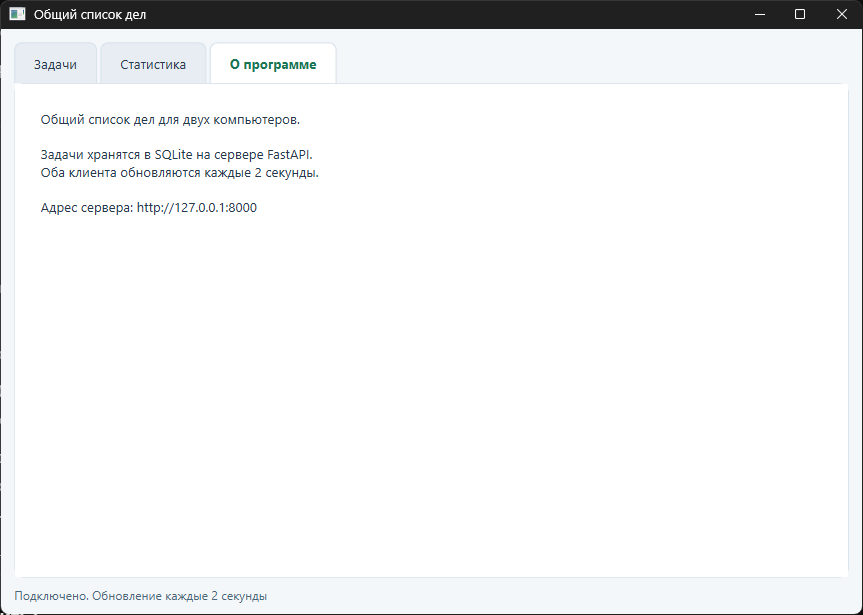
\includegraphics[width=.86\textwidth,height=.37\textheight,keepaspectratio]{figures/screenshots/about.png}
\caption{Вкладка «О программе» в работающем клиенте}
\label{fig:aboutwindow}
\end{figure}

Начальный размер окна составляет 780 на 530 пикселей. Элементы размещены в вертикальных и горизонтальных компоновщиках; при изменении размера окна область списка растягивается. Для вывода используется QListWidget: он позволяет связать строку с идентификатором задачи \cite{qtlist}. Благодаря этому одинаковые названия не мешают выбирать конкретную запись. Выделение сохраняется при обновлении списка, если выбранная задача ещё существует.

Для проверки совместной работы на одном компьютере запущены два отдельных окна клиента. После переименования задачи оба окна показывают запись «Запись к врачу в 19:00» (рисунок \ref{fig:twoclients}). Этот снимок подтверждает запуск двух экземпляров приложения и общее состояние списка на одном ПК; испытание связи между двумя физическими компьютерами проводится отдельно.

\begin{figure}[H]
\centering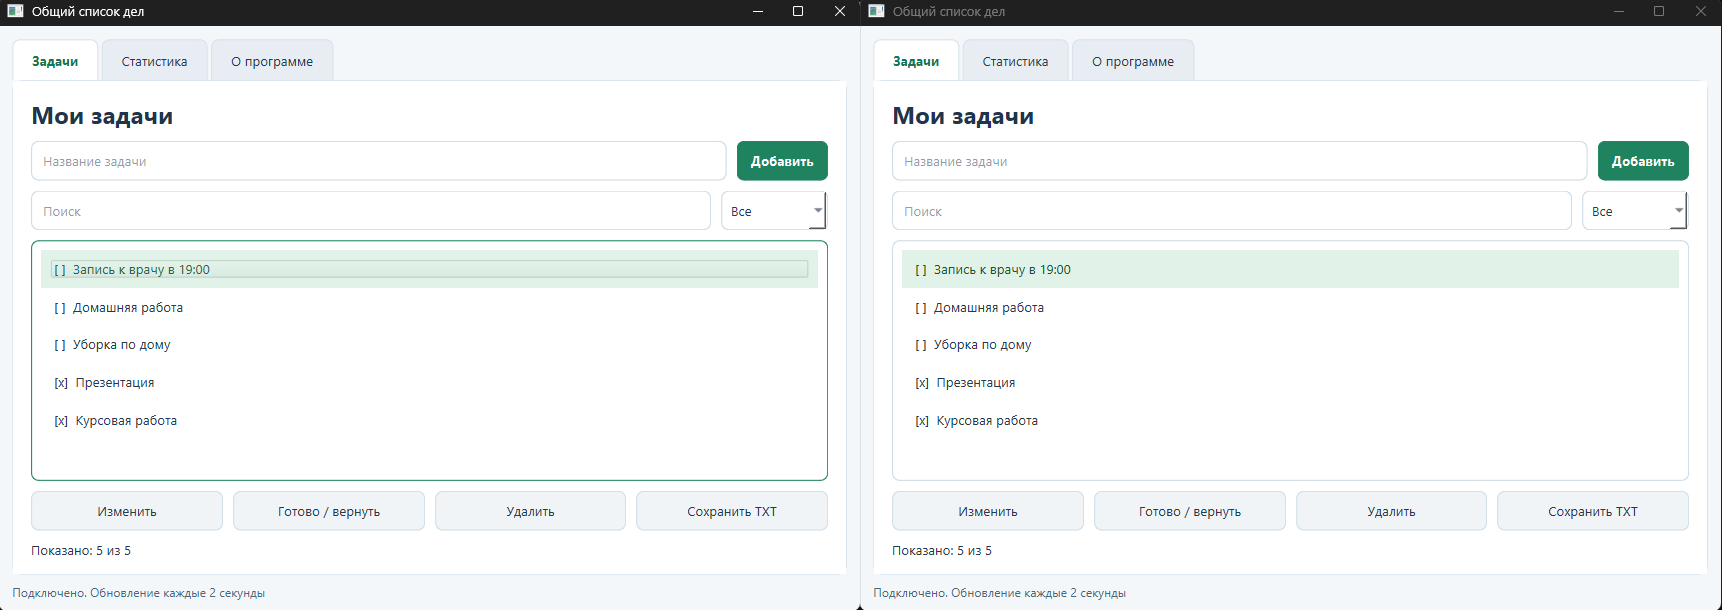
\includegraphics[width=.98\textwidth,height=.34\textheight,keepaspectratio]{figures/screenshots/two_clients.png}
\caption{Два клиента, запущенные на одном компьютере}
\label{fig:twoclients}
\end{figure}

Экспорт в TXT выполняется на компьютере пользователя. Программа записывает каждую задачу с отметкой [x] либо [ ] в отдельную строку. Используется кодировка UTF-8 с меткой BOM для корректного чтения русского текста в Блокноте Windows. На рисунке \ref{fig:exporttxt} показан файл, сохранённый из приложения и открытый в текстовом редакторе. Экспорт не меняет данные в SQLite.

\begin{figure}[H]
\centering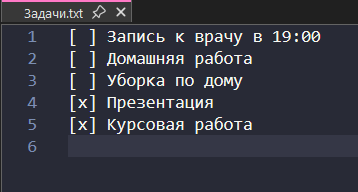
\includegraphics[width=.70\textwidth,height=.25\textheight,keepaspectratio]{figures/screenshots/export_txt.png}
\caption{Содержимое файла TXT после экспорта списка задач}
\label{fig:exporttxt}
\end{figure}

Если пользователь отменяет выбор файла, запись не выполняется. При ошибке сохранения появляется сообщение. При потере соединения с сервером клиент оставляет на экране последний полученный список и показывает в нижней строке состояние подключения. После восстановления связи список обновляется при следующем запросе.

\section{Проверка работы и сценарии приёмки}

Сервер проверялся на временной базе, не связанной с пользовательскими данными. Два экземпляра TestClient обращались к одной таблице и проверяли добавление, редактирование, переключение состояния, удаление и неверный ввод \cite{fastapitesting}. Затем тот же набор основных операций выполнялся через реально запущенный HTTP-сервер с двумя независимыми сеансами Requests. Проверки охватывали успешные операции, ошибочный ввод и сохранение записей. Эти испытания не использовали виджеты PySide6: проверялся обмен по HTTP и содержимое SQLite. Основные сценарии и ответы сервера приведены в таблице \ref{tab:autotests}.

\begin{table}[H]
\caption{Проверка основных HTTP-операций}
\label{tab:autotests}
\small\centering\renewcommand{\arraystretch}{1.22}
\begin{tabularx}{\textwidth}{|L{10mm}|Y|L{28mm}|}
\hline
№ & Проверяемое действие & Результат \\
\hline
1 & Получение пустого списка до добавления & HTTP 200; пустой список \\
\hline
2 & Создание задачи с русским названием & HTTP 200 \\
\hline
3 & Чтение новой задачи вторым тестовым клиентом & Запись найдена \\
\hline
4 & Редактирование названия и чтение первым клиентом & Новое название получено \\
\hline
5 & Изменение состояния и чтение первым клиентом & \texttt{done = true} \\
\hline
6 & Отклонение названия из пробелов & HTTP 400 \\
\hline
7 & Ошибка для отсутствующего идентификатора & HTTP 404 \\
\hline
8 & Удаление и повторное чтение & Запись отсутствует \\
\hline
9 & Открытие документации API & HTTP 200 \\
\hline
10 & Перезапуск HTTP-сервера с тем же файлом базы & Данные сохранены \\
\hline
\end{tabularx}
\end{table}

В таблице приведены операции серверной части. Поиск, фильтр, статистика и экспорт в TXT выполняются в клиентском окне и проверяются отдельно на Windows-ПК.

Один из сценариев включал следующую последовательность действий. Сначала сервер возвращает пустой список. Первый тестовый клиент отправляет название «Подготовить курсовую», после чего второй читает список и получает эту задачу. Второй клиент исправляет название и меняет состояние задачи на выполненное, а первый получает оба изменения при следующем чтении. После удаления оба видят пустой перечень. В этом примере проверяется совместное использование базы, а не скорость передачи данных.

Помимо основных операций проверена обработка неправильных запросов. В таблице \ref{tab:edgecases} приведены результаты повторной проверки, выполненной на временной базе без пользовательских данных.

\begin{table}[htbp]
\caption{Результаты проверки входных данных и запросов}
\label{tab:edgecases}
\small\centering\renewcommand{\arraystretch}{1.2}
\begin{tabularx}{\textwidth}{|L{47mm}|L{41mm}|Y|}
\hline
Проверяемое условие & Запрос & Фактический ответ \\
\hline
Название из пробелов & POST /tasks & HTTP 400 \\
\hline
Название из 121 символа & POST /tasks & HTTP 400 \\
\hline
Перевод строки и табуляция & POST /tasks & HTTP 400 \\
\hline
Несуществующий идентификатор & PATCH /tasks/999999 & HTTP 404 \\
\hline
Пустое название при редактировании & PATCH /tasks/1/title & HTTP 400 \\
\hline
Удаление отсутствующей задачи & DELETE /tasks/999999 & HTTP 404 \\
\hline
Название с апострофом & POST /tasks & HTTP 200, запись создана \\
\hline
Повторение названия & POST /tasks & HTTP 200, отдельная запись \\
\hline
\end{tabularx}
\end{table}

Проверки серверной части включали правильный ввод, ошибочные запросы, редактирование, отметки выполнения, удаление, получение изменений вторым HTTP-клиентом и сохранение SQLite после остановки сервера. В ходе проверки в Windows получены снимки главного экрана, статистики, редактирования, информационной вкладки, двух открытых клиентов и экспортированного текстового файла. Два окна работали на одном компьютере; проверка сетевого соединения между двумя физическими ПК остаётся отдельным сценарием из приложения Б.

\section{Ограничения программы}

Приложение не рассчитано на работу в публичной сети. На сервере отсутствуют вход пользователей и распределение прав. HTTP-запросы не шифруются, поэтому сервер следует запускать в доверенной локальной сети, не открывая порт для подключения из интернета.

При потере связи клиент оставляет на экране последний полученный список и сообщает, что связь с сервером отсутствует. Неотправленные действия не сохраняются. Текст новой задачи остаётся в поле ввода, чтобы пользователь мог повторить отправку после восстановления соединения. Следующий успешный опрос перечитает список.
